\chapter{Progress of Implementations}

\section{Basic MNIST classifier}
A basic MNIST classifier was constructed using Keras in Python. The classifier consisted of a single agent that trained on the dataset. The primary motivation for this approach was to establish a baseline for comparison with the performance of the SL algorithm. This solution was trained on a single GTX 1660. MNIST was picked as it is simple, well documented, and has a built in function in Keras to load it with minimal code. 

\section{Simple swarm learning}
In this experiment, a swarm of agents was created using the same model as that used in the Basic MNIST classifier. Each agent had access to the entire dataset for training, and all agents were able to communicate with each other. The agents operated in a loop, where they would each train for one epoch on their own copy of the training set, and then average their model weights with those of their neighbours. This implementation involved a total of five agents, who shared a single GTX 1660 among them. The graphs below depict the accuracy of an agent from the swarm, and also the accuracy of the lone agent.

\begin{figure}[h]
	\centering
	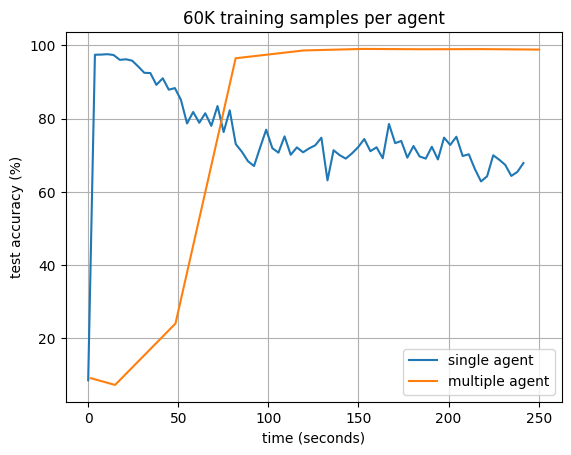
\includegraphics[width=0.5\textwidth]{accuracy_60k}
	\caption{Training accuracy over time for an agent from a swarm and a solo agent training with conventional methods, each agent has access to whole dataset.}
	\label{fig_60k}
\end{figure}

According to figure \ref{fig_60k}, at the outset, the swarm's accuracy took longer to converge to its highest value than that of the single agent algorithm, which may be attributed to the additional computational overhead associated with SL. After a certain period, the swarm's accuracy improved to the same level as that of the single agent. However, while the single agent began to exhibit signs of overfitting, the swarm's accuracy continued to increase. Ultimately, the swarm achieved a higher level of accuracy than the single agent.

It was observed that the agents achieved their final accuracy in a reduced number of training steps when their training loops were offset by even intervals of time. The author hypothesises that this may be due to the potential loss of training epochs when the agents' training is synced, as some of the agents may skip the most recent training when requesting updates.

\section{Reduced dataset swarm learning}
The focus of this experiment was to investigate the impact of reducing the amount of data available for training each agent. For this purpose, a fixed number of samples were randomly selected from the training set for each agent, and these samples were not altered throughout the training process. The experiment was conducted with 2000 and 500 samples per agent.

\begin{figure}[h]
	\centering
	\begin{subfigure}{.5\textwidth}
		\centering
		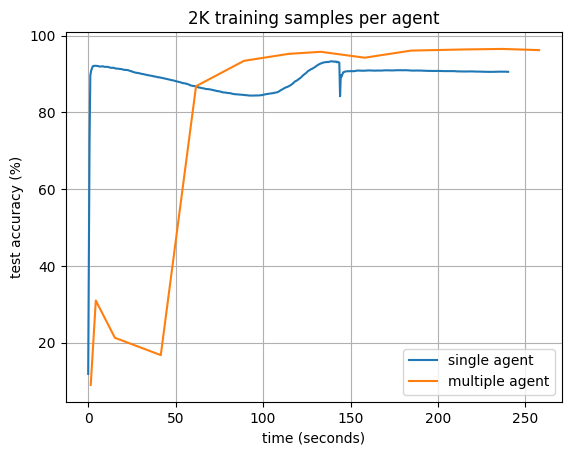
\includegraphics[width=\linewidth]{accuracy_2k}
		\caption{2000 samples per agent}
		\label{fig_2k}
	\end{subfigure}%
	\begin{subfigure}{.5\textwidth}
		\centering
		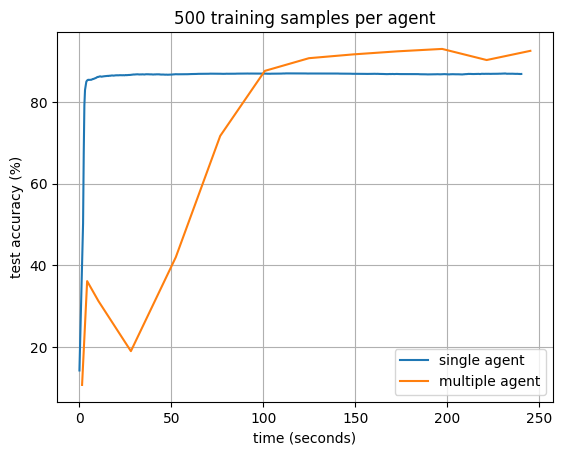
\includegraphics[width=\linewidth]{accuracy_500}
		\caption{500 samples per agent}
		\label{fig_500}
	\end{subfigure}
	\caption{Training accuracy over time for an agent from a swarm and a solo agent training with conventional methods, each agent has access to 2000 or 500 random samples from the dataset.}
	\label{fig_500_2k}
\end{figure}


As seem in figure \ref{fig_500_2k}, in both cases it was observed that the swarm required a longer time to reach its maximum accuracy. However, when it did, the swarm's peak accuracy exceeded that of the single agent by approximately 5\%-10\%. Both cases show a spike in accuracy near the start of swarm training, followed by a decrease in accuracy, and then a stable increase. This is likely due to the joining of new agents with untrained networks, which effectively add a random model to the pool of weights. A simple solution to this problem would be to have newly joined agents immediately request a model from their neighbouring agents and use that as their base network.